\documentclass[conference]{IEEEtran}
\IEEEoverridecommandlockouts

\usepackage{fancyhdr}
\pagestyle{fancy}
\fancyhf{}

\renewcommand{\thepage}{\Roman{page}} % Capital Roman numerals

\fancyhead[L]{\thepage}                 % Page number on left
\fancyhead[C]{S. VERMA, S. TULSYAN \& S. DHANUKA, A. SEN}

\usepackage{cite}
\usepackage{amsmath,amssymb,amsfonts}
\usepackage{algorithmic}
\usepackage{graphicx}
\graphicspath{{images/}}
\usepackage{textcomp}
\usepackage{xcolor}
\usepackage{booktabs}
\usepackage{multirow}

\newcommand{\Var}{\mathrm{Var}}
\newcommand{\R}{\mathbb{R}}

\begin{document}

\title{Quantitative Analysis of Media Bias and Stock Price Dynamics: The 2020 Shock}

\author{\small
\begin{minipage}[t]{0.48\textwidth}
\centering
Shivansh Verma \\
\textit{Dept of CS} \\
\textit{Ashoka University} \\
Sonipat, India \\
shivansh.verma\_ug2023@ashoka.edu.in
\end{minipage}
\hfill
\begin{minipage}[t]{0.48\textwidth}
\centering
Soham Tulsyan \\
\textit{Dept of CS} \\
\textit{Ashoka University} \\
Sonipat, India \\
soham.tulsyan\_ug2023@ashoka.edu.in
\end{minipage}
\\[0.6em]
\begin{minipage}[t]{0.48\textwidth}
\centering
Sashwat Dhanuka \\
\textit{Dept of CS} \\
\textit{Ashoka University} \\
Sonipat, India \\
sashwat.dhanuka\_ug2023@ashoka.edu.in
\end{minipage}
\hfill
\begin{minipage}[t]{0.48\textwidth}
\centering
Anirban Sen \\
\textit{Dept of CS} \\
\textit{Ashoka University} \\
Sonipat, India \\
anirban.sen@ashoka.edu.in
\end{minipage}
}

\maketitle

\thispagestyle{empty}

\begin{abstract}
% TODO: Abstract.
\end{abstract}

%=====================================================================
% INTRODUCTION  (1--1.25 pg)  --  Shivansh Verma, Soham Tulsyan, Sashwat Dhanuka
%   - Motivation: long para on why this is important / why we are doing this.
%   - What exactly we are doing: mention the RQs briefly.
%   - How: brief, high-level methodology; reasons behind VAR + regression.
%   - Findings: implications; brief basic accuracy metrics / aggregates;
%     mostly what we feel about the results.
%=====================================================================
\section{Introduction}

%=====================================================================
% RELATED WORK  (0.75--1 pg)  --  Shivansh Verma, Soham Tulsyan, Sashwat Dhanuka
%   - Cite at least 30 papers, 2022 onwards.
%   - Divide into 2--3 sections (e.g. by RQ or by theme).
%   - Frame a story per work: [author (cite) did xyz, found abc; pqr is the
%     gap; how our study differs; brief on their methodology].
%   - Answer: why are we doing this work (criticism + motivation).
%=====================================================================
\section{Related Work}

%=====================================================================
% DATA COLLECTION  (0.5--0.75 pg)
%=====================================================================
\section{Data Collection}

% Data source and format; scraping process, GDELT, MediaCloud; time span and
% volume of articles.  --  Shivansh Verma
\subsection{Corpus and Coverage}
Our object of study is the tone of the news that surrounds large United States
firms, so the corpus has to begin as close as possible to the full stream of that
coverage. We assemble it from MediaCloud, a service that continuously indexes the
output of national news outlets, and we query its United States national collection
one firm at a time over the period 2015 to 2025. Each query returns the news items
that name the firm, each carrying a publication date, a source outlet, and a
headline. We keep the headline as the unit of analysis, because the headline is the
one part of a news item written to compress the story's angle into a single line,
and it is therefore where a firm's coverage wears its stance most plainly. Cast this
way the net is deliberately wide: seeded with roughly $250$ large-capitalization
United States firms, the raw pull returns $6{,}284{,}404$ headlines, a stream large
enough that no single outlet or stretch of time dominates it.

A corpus of this size invites an obvious temptation, which is to make it larger
still, and we tested whether a second aggregator, GDELT, could extend the coverage
we had already gathered. It could not. The headlines GDELT returned were of visibly
poorer quality, often truncated or malformed and heavily duplicated across
near-identical records, so folding them into the corpus would have thinned a clean
signal with noise rather than deepening it. We keep the study on the MediaCloud
stream, whose headlines are consistently well formed and attributed, and treat that
stream as the raw material for everything that follows.

One feature of that raw material shapes every later choice. Coverage is spread
across firms with extreme inequality: a small number of the most heavily reported
names account for the bulk of all headlines, while a long tail of firms surfaces in
the news only occasionally. This unevenness is the first thing the data asks us to
confront once we begin turning a raw stream of headlines into a panel we can measure.

% Preprocessing, cleaning, filtering; relevance classifier as a black box
% ("we ran an RC to find financial articles of relevance about the companies
% considered"); rejected companies/articles.  --  Shivansh Verma, Sashwat Dhanuka
\subsection{Data Preprocessing}

\begin{figure}[t]
\centering
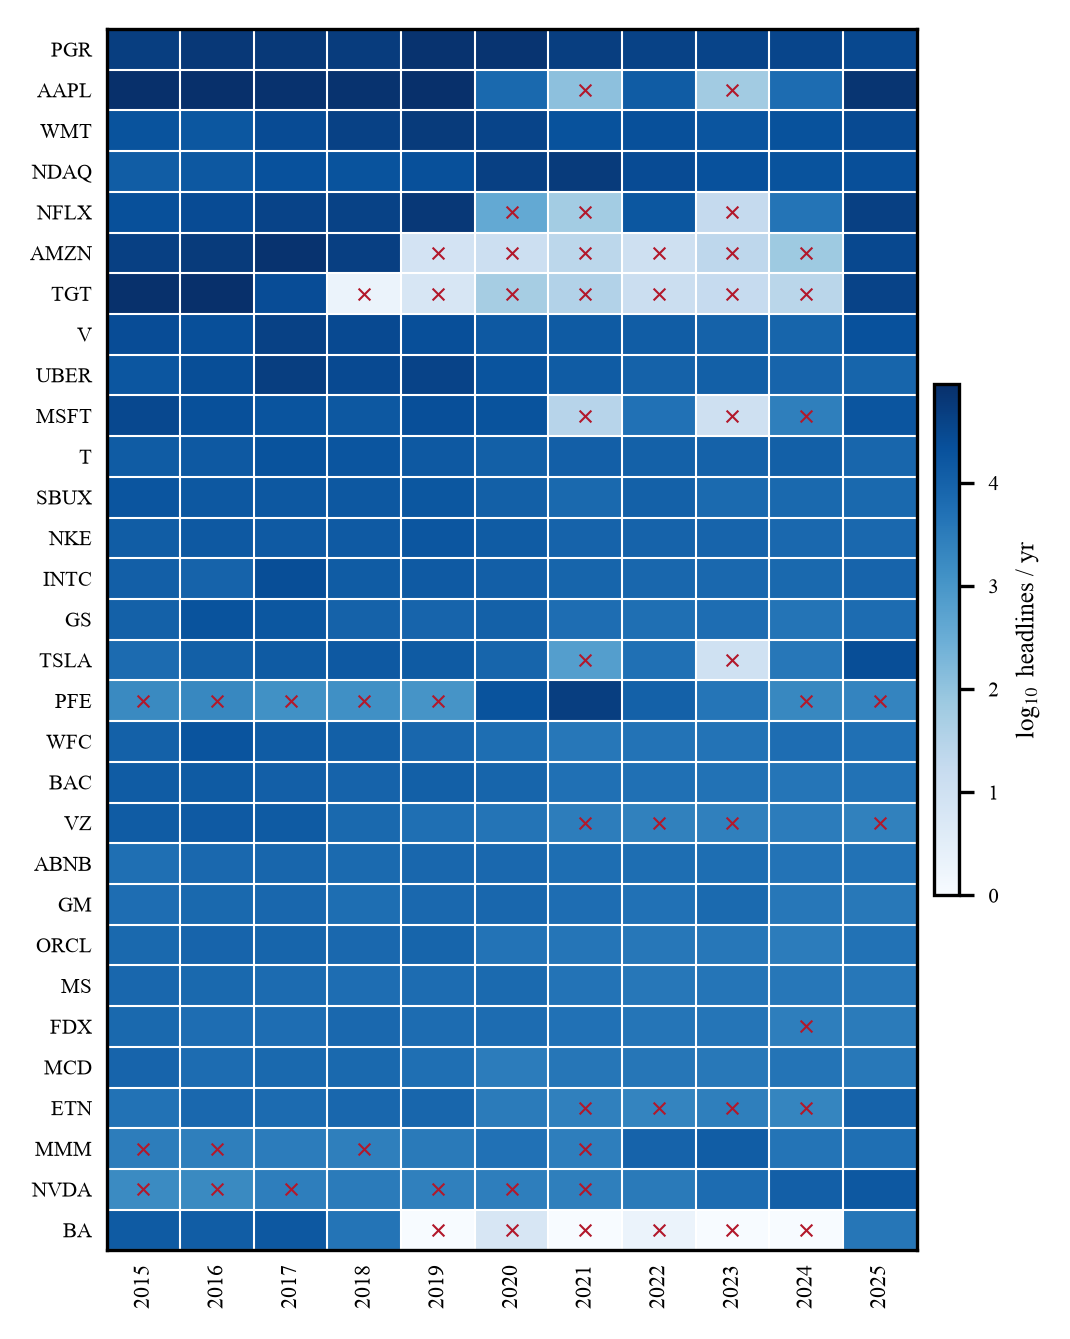
\includegraphics[width=\linewidth]{fig_stratification.png}
\caption{Yearly headline coverage for each candidate firm, shaded by
$\log_{10}$ headlines per year. A cross marks any year in which a firm sits at or
below the three-thousand-headline floor; a firm crossed in more than three of the
eleven years is set aside as too intermittently covered to support a continuous
series.}
\label{fig:strat}
\end{figure}

\begin{figure}[t]
\centering
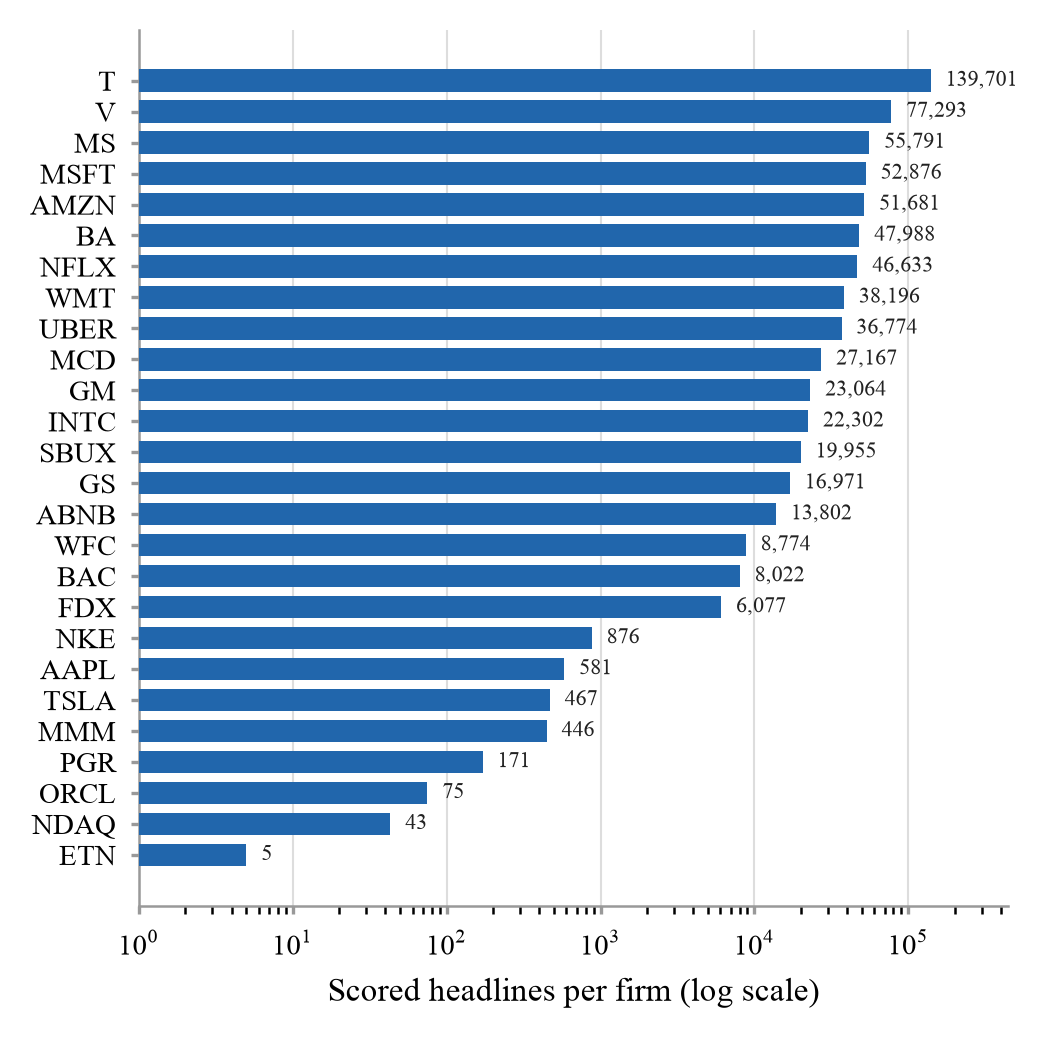
\includegraphics[width=\linewidth]{fig_coverage_per_firm.png}
\caption{Scored headlines per firm in the final corpus (26 firms, log scale).
Coverage spans more than four orders of magnitude, from AT\&T at $139{,}701$ down to
Eaton at $5$, which the firm fixed effects in the panel regressions absorb.}
\label{fig:coverage}
\end{figure}

The skew is not a nuisance to be smoothed away; it decides which firms can be
studied at all. A daily, firm-level measure of tone is only as steady as the
coverage beneath it, and a firm the news names a handful of times a month cannot
carry a daily series that means anything. We therefore keep the firms the press
reports on heavily and let the thin ones go. Ranking the universe by the volume of
coverage each firm attracts and holding onto the most reported names concentrates
the corpus onto its densely covered head, some $4{,}706{,}589$ headlines, and leaves
behind a long tail of firms that never generated enough news to measure.

Volume in a single year is not enough on its own, because coverage also has to
persist across the whole decade: a firm that falls quiet for years leaves stretches
of time that no series can span. We therefore hold each remaining firm to a floor of
more than three thousand headlines in a year, and set aside any firm that slips to or
below that floor in more than three of the eleven years from 2015 to 2025, since a
firm that runs thin that often cannot anchor a continuous weekly or daily series.
Figure~\ref{fig:strat} maps yearly coverage firm by firm and marks the years that
fall below the floor; the firms carried forward are those whose rows stay dark almost
throughout, while the ones that flicker pale in year after year are the ones the rule
removes.

Two kinds of contamination still sit inside what survives. A great many headlines
name a firm only in passing, in a list or an aside, while the story itself is about
something else; because a headline written about the firm almost always carries the
firm's name or its ticker symbol, we keep only the headlines that do and discard the
rest. The same wire report, in turn, is republished word for word across dozens of
outlets, so we collapse these near-identical copies to a single record per firm.
Table~\ref{tab:funnel} traces the corpus through these passes, from the full scrape
down to what remains: $695{,}731$ scored headlines across $26$ firms, each attached
to a firm the news followed closely and each naming that firm in its title. Even
within this retained set coverage stays strikingly unequal, spanning more than four
orders of magnitude from the most reported firm to the least
(Figure~\ref{fig:coverage}); the estimation later leans on firm-level effects
precisely so that these permanent differences in coverage volume cannot masquerade
as differences in tone.

\begin{table}[!htb]
\caption{From the full news scrape to the corpus the study runs on.}
\label{tab:funnel}
\centering
\small
\begin{tabular}{lrr}
\toprule
Stage & Headlines & Firms \\
\midrule
Full MediaCloud scrape & $6{,}284{,}404$ & $250$ \\
Most-covered firms retained & $4{,}706{,}589$ & $30$ \\
Name or ticker in title, de-duplicated & $695{,}731$ & $26$ \\
\bottomrule
\end{tabular}
\end{table}

% Table on article volume + temporal variation; final distribution/volume
% reported POST relevance classification.  --  Sashwat Dhanuka

%=====================================================================
% METHODOLOGY  (2--3 pg)
%=====================================================================
\section{Methodology}

% Only the final relevance classifier (mention failed experiments very briefly,
% if at all).  Report accuracy, precision, recall, F1.  Optional model-comparison
% graph/table (can go to appendix).  --  Sashwat Dhanuka
\subsection{Relevance Classification}

% For each RQ: hypothesis, null hypothesis, estimating equations, and a full,
% formal description of every variable (VIX, volume, etc.).  Brag about the work:
% assumption testing, normalization, regularization, etc.
%   RQ1, RQ2  --  Soham Tulsyan, Shivansh Verma
%   RQ3       --  Soham Tulsyan
\subsection{A Panel Design for the 2020 Break}
With a daily, firm-level stance series in hand and a matching series of daily stock
returns, the first question the 2020 shock raises is the plainest one: did either
series step to a new level once the shock arrived? The tempting way to answer it is
to average each series over the years before 2020 and over the years after, and read
off the difference. That answer would mislead, and seeing why fixes the design for
both questions that follow.

Two forces move a firm's coverage and its returns that have nothing to do with the
shock. Firms differ from one another in ways that hold across the whole sample: some
are simply covered more, and more warmly, than others, and some earn higher average
returns than others. And on any single day every firm is pushed in the same
direction by the news cycle and by the market as a whole. A raw before-and-after
average folds both of these into what it labels the ``2020 effect'': a shift in which
firms happen to be in the news, or a run of shared bad days, would surface as a break
that owes nothing to the shock itself.

A panel regression with two sets of fixed effects strips out exactly these two
confounders. Firm effects pin each firm to its own baseline, so the comparison is
between a firm and its own past rather than between one firm and another; time
effects hold constant whatever is common to every firm on a given day, or in a given
month, so a market-wide swing cannot be read as a firm-level break. What remains for
a post-2020 indicator to explain is the within-firm change net of common shocks,
which is exactly the quantity the shock question asks about. This is why we estimate
the break inside a two-way fixed-effects regression rather than from raw means, from a
single firm's time series, or from an event study around one date: only the panel
holds the standing differences between firms and the shared movements across them
fixed at the same time. The estimate is credible under three assumptions the setting
makes reasonable: that, absent the shock, the pre- and post-periods would have shared
a common trend; that the timing of the break is set by the pandemic's onset rather
than by anything in a firm's own coverage or returns; and that, after the
within-transformation, what is left is uncorrelated with the post indicator. To guard
the last of these we report HC1-robust standard errors throughout, and, where several
firms are covered on the same day, standard errors clustered by day.

\subsection{RQ1: Did Media Stance Shift After the Shock?}
The outcome for this question is the tone of a firm's coverage on a day. Each retained
headline is read by a target-dependent sentiment model that reports, for the firm
named in it, how likely its tone toward that firm is positive, negative, or neutral;
write these three probabilities as $p^{+}_a$, $p^{-}_a$, and $p^{0}_a$ for headline
$a$, with $p^{+}_a + p^{-}_a + p^{0}_a = 1$. We collapse them into a single signed
score, $p^{+}_a - p^{-}_a$, which runs from $-1$ for wholly unfavorable coverage to
$+1$ for wholly favorable coverage and sits near zero when the headline is even-handed
or the model is unsure. A firm's stance on a day is the average of these scores over
the headlines it drew that day,
\begin{equation}
\text{bias}_{it} = \frac{1}{N_{it}} \sum_{a \in A_{it}} \bigl(p^{+}_a - p^{-}_a\bigr),
\label{eq:bias}
\end{equation}
where $A_{it}$ is the set of retained headlines about firm $i$ on day $t$,
$N_{it} = |A_{it}|$ is that day's coverage volume, and
$\text{bias}_{it} \in [-1,1]$ is the average tone toward the firm.

We ask whether this daily stance moved to a new level after the shock. The regression
places stance on the post-2020 indicator alongside firm and daily time effects and the
day's coverage volume,
\begin{equation}
\text{bias}_{it} = \alpha_i + \delta_t^{\text{day}} + \beta\,\text{Post}_t
+ \gamma\,\text{vol}_{it} + \varepsilon_{it}.
\label{eq:rq1}
\end{equation}
Here $\text{Post}_t = \mathbf{1}[\,t \ge \text{2020-01-01}\,]$ switches on for every day
from January 2020 onward, and its coefficient $\beta$ is the quantity of interest;
$\alpha_i$ are the firm effects and $\delta_t^{\text{day}}$ the daily effects. The
control $\text{vol}_{it} = N_{it}$ enters because a daily average tightens
mechanically as more headlines are folded into it, so holding the count fixed keeps a
genuine change in tone from being mistaken for a change in the sheer amount of
coverage. We test
\begin{equation*}
H_0^{(1)}:\ \beta = 0 \qquad\text{against}\qquad H_1^{(1)}:\ \beta \neq 0,
\end{equation*}
estimating \eqref{eq:rq1} by the within-transformation with HC1-robust standard
errors, and, since several firms can be covered on the same day, reporting
day-clustered standard errors alongside them.

\subsection{RQ2: Did Firm-Level Returns Shift After the Shock?}
The second question asks the same of prices. The outcome is firm $i$'s daily log
return, $\text{return}_{it} = \ln P_{it} - \ln P_{i,t-1}$, where $P_{it}$ is the
firm's closing price on day $t$; we draw the daily closing prices, the S\&P~500 index,
and the VIX volatility index from \texttt{yfinance}. Log returns are additive over
time and roughly symmetric, which suits a linear model. Returns carry a large common
component---when the market rises, most firms rise with it---so the design must strip
that component out before it can see a firm-level break. Monthly time effects absorb
the broad market regime, and within each month the S\&P~500 return and the VIX account
for the day-to-day market swings and the level of volatility. The regression is
\begin{equation}
\text{return}_{it} = \alpha_i + \delta_t^{\text{month}} + \beta\,\text{Post}_t
+ \gamma_1\,\text{sp500\_ret}_t + \gamma_2\,\text{vix}_t + \varepsilon_{it},
\label{eq:rq2}
\end{equation}
with $\text{Post}_t$ as before, $\alpha_i$ the firm effects, $\delta_t^{\text{month}}$
the monthly effects, and $(\text{sp500\_ret}_t,\,\text{vix}_t)$ the market controls. We
again test the shock,
\begin{equation*}
H_0^{(2)}:\ \beta = 0 \qquad\text{against}\qquad H_1^{(2)}:\ \beta \neq 0,
\end{equation*}
estimating \eqref{eq:rq2} by the within-transformation with HC1-robust standard errors.
Table~\ref{tab:variables} gathers every quantity that enters the two regressions, so
that the returns model in particular is read as the post indicator and the market
controls acting together rather than any one of them alone.

\begin{table*}[!t]
\centering
\small
\caption{Variables in the RQ1 (stance) and RQ2 (returns) regressions.}
\label{tab:variables}
\begin{tabular}{p{2.6cm}p{1.4cm}p{8.4cm}}
\toprule
\textbf{Variable} & \textbf{Used in} & \textbf{Meaning} \\
\midrule
$\text{bias}_{it}$ & RQ1 (dep.) & Daily firm stance: the signed mean $p^{+}_a-p^{-}_a$ of the headlines about firm $i$ on day $t$. \\
$\text{return}_{it}$ & RQ2 (dep.) & Daily log return of firm $i$, $\ln P_{it}-\ln P_{i,t-1}$. \\
$\text{Post}_t$ & RQ1, RQ2 & Shock indicator, $\mathbf{1}[t\ge\text{2020-01-01}]$; its coefficient $\beta$ is the parameter of interest. \\
$\text{vol}_{it}$ & RQ1 & Coverage volume: the number of retained headlines about firm $i$ on day $t$. \\
$\text{sp500\_ret}_t$ & RQ2 & Daily S\&P~500 index return, controlling for broad market movement. \\
$\text{vix}_t$ & RQ2 & Daily VIX level, controlling for market volatility. \\
$\alpha_i$ & RQ1, RQ2 & Firm effects, absorbing permanent differences across firms. \\
$\delta_t^{\text{day}}$ & RQ1 & Daily effects, absorbing shocks common to all firms on a day. \\
$\delta_t^{\text{month}}$ & RQ2 & Monthly effects, absorbing shocks common to all firms in a month. \\
\bottomrule
\end{tabular}

\vspace{2pt}
{\footnotesize \textit{Note:} ``(dep.)'' marks the dependent variable; the remaining rows are regressors or fixed effects.}
\end{table*}

\subsection{RQ3: }

%=====================================================================
% RESULTS  (2--3 pg)
%   Add VAR/regression plots here. Distinguish method plots from finding plots.
%=====================================================================
\section{Results}

% Regression table, final finding, hypothesis testing.  --  Shivansh Verma
\subsection{RQ1: No Detectable Shift in Media Stance}
Estimating \eqref{eq:rq1} on the $27{,}627$ firm-day stance observations---$26$ firms
across $3{,}982$ trading days---returns the coefficients in
Table~\ref{tab:results}(a). The post-2020 coefficient is $\hat{\beta} = +0.011$ with
an HC1 standard error of $0.030$ ($p = 0.71$), and clustering by day barely disturbs
it ($\text{SE} = 0.030$, $p = 0.72$), so the within-day dependence between firms is
not hiding a result. We cannot reject $H_0^{(1)}$: once each firm is set against its
own history and the day's common movement is held fixed, the tone of coverage does not
step to a new level after the shock. The volume control behaves exactly as its purpose
demands---its coefficient is $-0.0038$ ($p < 0.001$), so the days on which a firm is
most heavily covered are the days its average tone is pulled back toward neutral, the
mechanical averaging effect the control exists to absorb. The within $R^2$ of $0.002$
is what one expects when a single firm's day-to-day tone is dominated by the noise of
individual headlines. A null here is not a failure to find something; it says the shock
left no common, firm-level mark on tone once the news cycle's own daily swings are
taken out.

% --  Shivansh Verma
\subsection{RQ2: No Detectable Shift in Firm-Level Returns}
The same estimation on returns, \eqref{eq:rq2} over $20{,}537$ firm-day observations,
tells the matching story (Table~\ref{tab:results}(b)). The post-2020 coefficient is
all but zero, $\hat{\beta} = -0.0001$ ($\text{SE} = 0.0013$, $p = 0.92$): returns show
no level break either. What the regression does register is the market itself. The
S\&P~500 return enters with a coefficient of $1.10$ ($p < 0.001$)---the familiar market
beta near one---and together with the monthly effects it accounts for about a third of
the within-firm variation in returns ($R^2 = 0.32$). Volatility adds nothing once the
market return is present ($\text{VIX}$, $p = 0.68$). The reading echoes RQ1: firm
returns move with the market, as they always have, but the shock itself leaves no
separate firm-level step behind. Taken together the two nulls are informative rather
than empty---after common shocks are removed, neither the tone of coverage nor firm
returns jumped in 2020. A level test is not the only way the shock could have mattered,
though: it could have changed how tone and returns move \emph{with one another} over
time rather than where each of them sits, and a static regression cannot see that.

\begin{table}[t]
\caption{Regression results for RQ1 (stance, Eq.~\ref{eq:rq1}) and RQ2 (returns, Eq.~\ref{eq:rq2}). Both fail to reject the null of no post-2020 level shift once common daily (RQ1) and monthly (RQ2) shocks are absorbed.}
\label{tab:results}
\centering
\small
\textbf{(a) RQ1 --- Daily Stance} (firm $+$ day FE, HC1 SE)\\[3pt]
\begin{tabular}{lrrr}
\toprule
Variable & Coef. & SE & $p$ \\
\midrule
Post ($\hat{\beta}$) & $+0.01096$ & $0.02964$ & $0.712$ \\
Article volume       & $-0.00381$ & $0.00049$ & $<0.001$ \\
\midrule
\multicolumn{4}{l}{$n=27{,}627$;\ 26 firms;\ 3,982 days;\ within $R^2=0.0017$} \\
\multicolumn{4}{l}{day-clustered $p_{\text{Post}}=0.717$} \\
\bottomrule
\end{tabular}

\vspace{7pt}
\textbf{(b) RQ2 --- Daily Returns} (firm $+$ month FE, HC1 SE)\\[3pt]
\begin{tabular}{lrrr}
\toprule
Variable & Coef. & SE & $p$ \\
\midrule
Post ($\hat{\beta}$) & $-0.00013$ & $0.00132$ & $0.921$ \\
S\&P 500 return      & $+1.09876$ & $0.01869$ & $<0.001$ \\
VIX                  & $-0.00003$ & $0.00006$ & $0.684$ \\
\midrule
\multicolumn{4}{l}{$n=20{,}537$;\ 26 firms;\ within $R^2=0.316$} \\
\bottomrule
\end{tabular}
\end{table}

% --  Soham Tulsyan
\subsection{RQ3: }

%=====================================================================
% DISCUSSION  (0.75--1.25 pg)  --  Soham Tulsyan, Sashwat Dhanuka
%   Subsection per RQ, 3 paras each:
%     Para 1: implication of findings.
%     Para 2: limitations / what we did not observe or consider.
%     Para 3: future work / how to extend.
%=====================================================================
\section{Discussion}

\subsection{RQ1: }

\subsection{RQ2: }

\subsection{RQ3: }

%=====================================================================
% CONCLUSION  (0.25 pg)  --  Soham Tulsyan, Shivansh Verma, Sashwat Dhanuka
%   Summary of what we did, how, and the findings. 1--2 paras max.
%=====================================================================
\section{Conclusion}

%=====================================================================
% APPENDIX (optional)
%=====================================================================
% \appendix

%=====================================================================
% BIBLIOGRAPHY  (@misc entries; target >= 30 papers, 2022 onwards)
%=====================================================================
% References: add BibTeX @-entries to references.bib, cite them with \cite{key}
% in the text (target >= 30, mostly 2022 onwards), then uncomment the two lines
% below to render the bibliography.
% \bibliographystyle{IEEEtran}
% \bibliography{references}

\end{document}
